%\documentclass[12pt,fleqn, leqno, acm]{article}
\documentclass[12pt]{article}

%% Estilos e Plug-Ins
%\usepackage{a4wide}
\usepackage{a4}
\ifx\pdfoutput\undefined
   \usepackage[dvips]{graphicx}
\else
   \usepackage[pdftex]{graphicx}
\fi
\usepackage{times}
\usepackage{isolatin1}
\usepackage[brazil]{babel}
\usepackage{fancyheadings}
\usepackage{lastpage} 

\pagestyle{fancy}

\textheight=8.2in
%\headwidth=1.2\textwidth
\lhead{\setlength{\unitlength}{1mm} 
\begin{picture}(0,0) 
\put(5,0){
\includegraphics[width=0.8in]{figs/fundacao.pdf}} 
\end{picture}} 
\chead{}
\rhead{\setlength{\unitlength}{1mm} 
\begin{picture}(0,0) 
\put(5,0){
\includegraphics[width=0.8in]{figs/tecgraf.pdf}} 
\end{picture}} 

\lfoot{\scriptsize %
Tecgraf/PUC-Rio \hfill -
\hfill Rua Marqu�s de S�o Vicente, 225 - Pr�dio Velloso \hfill -
\hfill CEP 22453-900 \hfill - \hfill Rio de Janeiro -- Brasil\\
Tel. +55 21 512-5984 - Fax. +55 21 259-2232 \hfill -
\hfill E-mail: openbus@tecgraf.puc-rio.br \hfill -
\hfill URL: http://www.tecgraf.puc-rio.br\\
\vspace{0.5cm} 
\today \hfill P�gina \thepage \hspace{0.1cm} de \pageref{LastPage}} 
%27/6/2006	P�ina 1 de 33
\cfoot{}
\rfoot{}

\addtolength{\parskip}{\baselineskip}

%\hyphenation{
%in-te-gra-\c{c}\~oes
%apli-ca-\c{c}\~oes
%}

% ===================
% In�io do documento
% ===================
\begin{document}

\title{OpenBus}
\author{}
\date{}
\maketitle
\thispagestyle{empty}

\section{Introdu��o}
\label{introducao}

Os profissionais da �rea de Explora��o e Produ��o da Petrobras utilizam
 diversas aplica��es computacionais no desempenho de suas atividades t�cnicas.
Por exemplo, as tarefas relacionadas � aquisi��o, processamento e interpreta��o
 de dados s�smicos exigem a participa��o de diferentes profissionais, e cada
 profissional pode necessitar de v�rias aplica��es.
O fato de uma �nica aplica��o n�o dar suporte a todas as fases do trabalho e,
 �s vezes, nem mesmo a uma fase inteira, � fruto da elevada complexidade
 t�cnica inerente � manipula��o desses dados.
Essa complexidade se reflete diretamente nas aplica��es, for�ando um alto grau
 de especializa��o, e praticamente torna imposs�vel a constru��o de uma
 aplica��o que permeie todas as fases de trabalho sobre um dado.

Uma decorr�ncia direta dessa pluralidade de aplica��es utilizadas para a
 manipula��o de um dado � a necessidade de integra��o.
Afinal, para que o trabalho seja realizado, � preciso que os dados sejam
 migrados de uma aplica��o para outra, at� que o resultado final seja
 alcan�ado.
Em resumo, a capacidade de integra��o entre aplica��es � um suporte essencial
 para o trabalho dos profissionais da �rea de E\&P.

Ao longo de um ciclo de trabalho, um profissional carrega um dado em uma
 aplica��o e, atrav�s das funcionalidades providas por esta aplica��o, manipula
 o dado como necess�rio.
Em uma situa��o t�pica, o profissional manipula o dado at� o limite oferecido
 pela aplica��o e, ent�o, transporta o dado para outra aplica��o de forma a
 continuar seu trabalho.
Entretanto, na pr�tica, essa troca de dados entre duas aplica��es n�o
 necessariamente � feita de forma simples ou at� mesmo satisfat�ria.

Diferentes aplica��es da �rea de E\&P possuem formas pr�prias de representar e
 armazenar os dados.
Al�m disso, a quantidade e a variedade de atributos e meta-informa��es
 relacionadas a um mesmo tipo de dado tamb�m podem ser diferentes.
A falta de padroniza��o gera dificuldades na troca de dados entre as aplica��es
 que, muitas vezes, acaba sendo feita manualmente pelo pr�prio usu�rio.
A integra��o manual consiste na exporta��o dos dados em algum formato
 padronizado de arquivo na aplica��o de origem, a carga desse arquivo na
 aplica��o destino e os ajustes necess�rios para que eventuais informa��es
 adicionais, n�o representadas no arquivo gerado, sejam criadas corretamente no
 destino.
Essa forma de integra��o � fraca, pois obriga o usu�rio a assumir o papel de
 integrador e abre a possibilidade de perda das informa��es que porventura n�o
 sejam representadas no formato de arquivo utilizado.
Em uma situa��o extrema, as aplica��es podem n�o compartilhar um formato comum
 de arquivo, o que pode inviabilizar a troca de dados entre elas.

Quando as aplica��es s�o desenvolvidas internamente pela Petrobras, ou possuem
 c�digo aberto, ou, ainda, disp�em de interfaces para programa��o de extens�es,
 a integra��o por ser feita de forma program�tica direta.
Essa integra��o {\em ad hoc} entre duas aplica��es facilita substancialmente o
 trabalho do usu�rio que, ao inv�s de trocar arquivos e configura��es entre as
 aplica��es, apenas comanda a transfer�ncia dos dados.
Al�m disso, a integra��o program�tica pode considerar, al�m dos dados, os
 atributos e meta-informa��es que sejam comuns, ou convert�veis, entre as
 aplica��es, maximizando a qualidade do dado trocado e diminuindo as eventuais
 perdas de informa��es desse processo.
Essa forma de integra��o tamb�m est� presente, eventualmente, entre aplica��es
 de um mesmo fabricante, como � o caso das aplica��es de geologia e geof�sica
 da Landmark.

Dois exemplos de integra��o program�tica direta entre aplica��es pr�prias da
 Petrobras s�o a integra��o v3o2/WebSintesi e a WebSintesi/SIGEO.
A integra��o v3o2/WebSintesi � feita atrav�s de uma interface de acesso � �rea
 de projetos pr�pria do WebSintesi que � acessada pelo v3o2.
Dessa forma, o v3o2 tem acesso aos projetos do WebSintesi, podendo ler e
 escrever arquivos nos projetos.
A integra��o WebSintesi/SIGEO � feita de forma an�loga: uma interface de acesso
 espec�fica para aos projetos do SIGEO � acessada pelo WebSintesi que, atrav�s
 dela, consegue criar novos objetos nos projetos SIGEO.

A integra��o direta entre aplica��es �, sem d�vida, melhor do que a integra��o
 externa, feita pelo usu�rio atrav�s da troca de arquivos e ajustes manuais.
Entretanto, o esfor�o necess�rio na infra-estrutura para integrar as aplica��es
 � muito grande, pois precisamos codificar uma {\em ponte} espec�fica para
 ligar cada par de aplica��es.
Isso nos leva a um n�mero quadr�tico de codifica��es de pontes em rela��o ao
 n�mero de aplica��es.
A cada nova aplica��o a ser integrada, � preciso codificar uma ponte que
 integre esta nova aplica��o com cada uma das aplica��es j� existentes, o que
 significa (\(\frac{n(n-1)}{2}\)) codifica��es para {\em n} aplica��es.
Por exemplo, para integrar 10 aplica��es precisamos codificar 45 pontes.

Se a integra��o direta entre os pares de aplica��es demanda um esfor�o muito
 elevado, a ado��o de aplica��es de um mesmo fabricante, que possuem
 funcionalidades de integra��o intr�nsecas, � direta mas insuficiente.
Afinal, nenhum fabricante possui um conjunto de aplica��es que atenda a
 totalidade das funcionalidades exigidas pelos profissionais nos seus ciclos de
 trabalho.
Por outro lado, mesmo que um fabricante possu�sse tal conjunto de aplica��es,
 dificilmente sua ado��o seria desej�vel, dada a total depend�ncia que se
 estabeleceria deste fabricante.

Uma abordagem alternativa para as integra��es externa (via arquivos) e direta
 (via pontes entre os pares) � a ado��o de uma plataforma comum de integra��o
 entre aplica��es.
O princ�pio b�sico de uma plataforma de integra��o � definir um componente ou
 um {\em barramento} comum atrav�s do qual todas as aplica��es possam trocar
 dados.
Nesse modelo, cada aplica��o se conecta ao barramento, segundo um protocolo
 pr�prio deste barramento, e carrega ou exporta dados para outras aplica��es
 tamb�m conectadas ao barramento.

Como na integra��o direta, � necess�rio codificar uma ponte para conectar cada
 aplica��o ao barramento.
Tamb�m como na integra��o direta, o fato de se estabelecer uma interface e de
 se codificar uma ponte espec�fica, permite maximizar a qualidade do dado
 trocado entre as aplica��es, minimizando a eventual perda de informa��es
 decorrente da heterogeneidade dessas aplica��es.
Por outro lado, como o barramento define uma linguagem comum entre todas as
 aplica��es, a codifica��o de uma ponte entre uma aplica��o e o barramento � o
 suficiente para que esta aplica��o se integre a todas as demais aplica��es
 conectadas ao barramento.
Ou seja, diferente da abordagem de integra��o direta, onde o esfor�o de
 infra-estrutura � quadr�tico, a integra��o por meio de um barramento exige um
 esfor�o linear em fun��o do n�mero de aplica��es.
De fato, para integrar {\em n} aplica��es, � preciso codificar apenas {\em n}
 pontes.

Outra vantagem significativa da integra��o atrav�s de um barramento comum � a
 possibilidade de criarmos {\em liga��es ativas} entre as aplica��es.
Uma liga��o ativa � uma liga��o atrav�s da qual uma aplica��o pode perceber
 mudan�as nos dados de outra aplica��o.
Ou seja, por meio de uma liga��o ativa duas aplica��es podem trocar mensagens
 ao inv�s de apenas dados.
Atrav�s das liga��es ativas podemos criar integra��es onde as aplica��es
 trocam informa��es dinamicamente, � medida em que o usu�rio interage com cada
 uma.
Por exemplo, se uma aplica��o permite a visualiza��o de um dado proveniente de
 outra aplica��o, � poss�vel refletir na tela uma modifica��o que seja feita no
 dado original imediatamente ap�s essa modifica��o ter sido feita na aplica��o
 que hospeda esse dado.
Al�m disso, podemos explorar essa forma de comunica��o entre as aplica��es
 para, por exemplo, permitir o trabalho colaborativo entre usu�rios.

Na �rea de E\&P, existem solu��es de mercado que implementam arquiteturas de
 integra��o de aplica��es.
Entretanto, como veremos na se��o seguinte, essas solu��es s�o limitadas e n�o
 atendem a todos os requisitos de integra��o do E\&P da Petrobras.
Em fun��o dessas limita��es, e do fato desta abordagem de integra��o se mostrar
 como a mais adequada, n�s propomos, neste documento, a constru��o de uma
 arquitetura de integra��o baseada em um barramento, que chamamos de OpenBus.

Na se��o seguinte, al�m da apresenta��o e da an�lise das solu��es de mercado,
 n�s apresentamos as tecnologias que podem ser utilizadas na constru��o de uma
 arquitetura de integra��o e avaliamos cada uma em fun��o dos requisitos
 impostos pelas aplica��es de E\&P.
Na se��o \ref{arquitetura}, n�s descrevemos a arquitetura OpenBus,
 explicitando os requisitos contemplados e detalhando os servi�os que ser�o
 providos pela arquitetura.
Por fim, na se��o \ref{conclusoes}, conclu�mos este documento, sintetizando
 os benef�cios da arquitetura proposta.



\section{Estado da arte}
\subsection{Solu��es de mercado para a integra��o de dados e aplica��es de E\&P}
A solu��o para a integra��o de aplica��es de E\&P mais abrangente dispon�vel
no mercado � a plataforma OpenSpirit. O desenvolvimento dessa plataforma resultou de um cons�rcio
(a OpenSpirit Alliance),
que uniu esfor�os de diferentes companhias de petr�leo e fabricantes de
software para a defini��o de um {\em framework} de integra��o de aplica��es
que suportasse tanto o compartilhamento de dados mantidos em diferentes
reposit�rios, 
como tamb�m a colabora��o entre diferentes aplica��es.
Esse {\em framework} � comercializado hoje por uma companhia de software
independente (a OpenSpirit Foundation), que conta com um grupo de investidores
que inclui tanto companhias de petr�leo, como Chevron e Shell, como tamb�m
provedores de software e servi�os, como Schlumberger e Paradigm.

O {\em framework} OpenSpirit � composto por tr�s elementos principais:
o OpenSpirit Runtime, conectores de dados (Data Connectors)
e adaptadores de aplica��es (Application Adapters).
\begin{itemize}
\item OpenSpirit Runtime

O OpenSpirit Runtime prov� a infraestrutura de suporte para a integra��o de 
aplica��es e dados. Essa infraestrutura oferece uma s�rie de servi�os 
utilizados pelos
conectores de dados e adaptadores de aplica��es, como, 
por exemplo, a conex�o de uma aplica��o ao ambiente
de integra��o, a disponibiliza��o de informa��es sobre os reposit�rios de
dados acess�veis, e a difus�o de mensagens (eventos de colabora��o) entre
aplica��es. 

Para garantir a independ�ncia da plataforma de execu��o e da linguagem de
desenvolvimento das aplica��es 
--- um requisito essencial � ampla interoperabilidade pretendida 
pelo {\em framework} ---
a infraestrutura de suporte de integra��o implementada pelo OpenSpirit
� baseada no {\em middleware} CORBA, e em alguns dos servi�os padronizados
para sua arquitetura.

\item Conectores de Dados

Conectores de dados, ou {\em data servers}, s�o os elementos respons�veis por
implementar os servi�os de acesso aos diferentes reposit�rios, ou
{\em datastores}.
Esses conectores prov�em �s aplica��es uma vis�o uniforme e homog�nea dos
dados acessados, independente dos formatos internos adotados
por um cada tipo de reposit�rio.
Essa vis�o uniforme � baseada em um modelo de dados gen�rico 
(OpenSpirit Data Model),
oferecido pelos conectores de dados em sua interface de acesso;
� responsabilidade de cada tipo de conector realizar o mapeamento desse modelo
para um reposit�rio espec�fico.

� importante observar que o modelo de dados atualmente implementado 
pela OpenSpirit
� restrito ao dom�nio da Geologia e Geof�sica, o que impede
a integra��o de aplica��es de outros dom�nios, como Engenharia
e Qu�mica.
Al�m disso, apenas a pr�pria OpenSpirit desenvolve e comercializa 
conectores de dados; n�o existe um {\em toolkit} para o desenvolvimento
desses conectores.
Essa restri��o impede que reposit�rios de dados providos
por aplica��es e sistemas desenvolvidos pela Petrobras sejam incorporados
ao ambiente de integra��o, a menos que a pr�pria OpenSpirit seja
contratada para desenvolver os conectores necess�rios.

A OpenSpirit disponibiliza, atualmente, conectores 
para os seguintes reposit�rios: Open\-Works/Seisworks, GeoFrame/IESX/Charisma,
Finder,
GOCAD, Kingdom, Petra,
Managed SEGY (dados SEGY 2D e 3D armazenados em um sistema de arquivos),
Recall e ArcSDE.
Contudo, conectores espec�ficos podem n�o suportar
todos os tipos de dados de um reposit�rio;
o conector para o GOCAD, por exemplo, oferece por enquanto apenas o acesso a 
volumes s�smicos. 

\item Adaptadores de Aplica��es

Adaptadores de aplica��es (ou {\em application plug-ins}),
s�o os componentes respons�veis por integrar as diferentes aplica��es
ao ambiente OpenSpirit.
Esses componentes utilizam a
API oferecida pelo {\em toolkit} de desenvolvimento
para prover �s aplica��es o acesso aos servi�os de dados e de 
colabora��o disponibilizados pelo {\em framework}.
O {\em toolkit} de desenvolvimento � 
dispon�vel atualmente para diferentes linguagens (Java, C++, C\#, VB, Delphi)
e plataformas (Windows, Solaris, Linux, Irix).
Diversos fornecedores de software, como Schlumberger (Petrel),
Landmark (OpenWire), Earth Decision (Gocad) e Hampson-Russell (AVO),
prov�em adaptadores para suas aplica��es.
A pr�pria Petrobras � licenciada como desenvolvedor OpenSpirit,
e est� implementando para o WebSintesi/VGE
o acesso, via {\em framework} OpenSpirit, a reposit�rios de dados como 
Open\-Works/Seisworks e GeoFrame/IESX.

Como vimos anteriormente, os servi�os de acesso a dados s�o
oferecidos por conectores espec�ficos para cada reposit�rio.
Atrav�s de um mecanismo de {\em query} oferecido pela API, aplica��es podem 
criar, ler, atualizar
e remover dados com base no modelo de dados gen�rico oferecido por
esses conectores.
O mecanismo de {\em query}, contudo, n�o permite o acesso a {\em bulk data}, 
como volumes s�smicos e horizontes 3D. Para esse tipo de acesso, 
a API prov� a representa��o dos dados como objetos remotos.

A colabora��o entre aplica��es � baseada em 
um servi�o de difus�o de mensagens (notifica��es),
oferecido pelo OpenSpirit Runtime.
Esse servi�o permite que aplica��es 
que operam sobre um mesmo conjunto de dados
compartilhamem {\em eventos} 
de intera��o de usu�rio (sele��o e altera��o de dados, movimenta��o de cursor,
defini��o de �reas de interesse).
A API provida pelo {\em toolkit} oferece mecanismos para que as aplica��es
possam gerar e receber esses eventos, encapsulando o acesso ao
servi�o de notifica��es.

Um fator limitante para a colabora��o entre aplica��es atrav�s do 
{\em framework} � a restri��o do escopo dessa colabora��o
a uma sess�o OpenSpirit. Essa sess�o, determinada no momento de conex�o 
da aplica��o ao ambiente, estabelece tamb�m
o conjunto de dados, ou projetos ({\em ProjectSet}) acess�veis 
pela aplica��o durante a conex�o.
No ambiente de integra��o OpenSpirit, cada usu�rio ({\em userid}) � 
associado a uma configura��o particular, que inclui a defini��o das sess�es
�s quais as aplica��es iniciadas por esse usu�rio poder�o conectar-se.
Como sess�es n�o s�o compartilhadas entre usu�rios, n�o h� colabora��o entre
aplica��es iniciadas por usu�rios diferentes.

Al�m de eventos de colabora��o, o {\em framework} OpenSpirit permite 
que aplica��es recebam notifica��es de eventos de altera��o dos dados 
de um reposit�rio (cria��o, altera��o e remo��o),
enviada pelos conector correspondente.
Essa facilidade depende da capacidade do conector 
gerar esse tipo de evento; atualmente, apenas os conectores OpenWorks e Geoframe
possuem essa capacidade.

\end{itemize}
Uma outra solu��o dispon�vel no mercado para a integra��o de aplica��es e
reposit�rios de dados de E\&P � o PowerHub, comercializado pela Landmark.
Assim como o modelo de dados gen�rico implementado pelo {\em framework}
OpenSpirit, a plataforma PowerHub oferece um modelo de dados 
que abstrai formas de armazenamento propriet�rias,
permitindo �s aplica��es acessar de maneira uniforme dados providos 
por diferentes reposit�rios.

Diferentemente do {\em framework} OpenSpirit, � poss�vel desenvolver
conectores para a integra��o de reposit�rios de dados � plataforma PowerHub, o
que, em princ�pio, permitiria a integra��o de dados disponibilizados por
aplica��es e sistemas desenvolvidos pela Petrobras.
Contudo, a API para acesso aos reposit�rios
consiste apenas de uma interface de
{\em query} para acesso a bases de dados, baseada em Java JDBC;
essa API n�o oferece acesso a {\em bulk data}, como volumes s�smicos.
Para acessar esse tipo de dado, � necess�rio que as aplica��es implementem
seus pr�prios mecanismos, baseados em {\em toolkits} providos
pelos fornecedores das aplica��es que mant�m os reposit�rios.

Uma outra restri��o com respeito ao uso da plataforma PowerHub
como solu��o de integra��o de aplica��es e dados de E\&P � a imposi��o do 
uso da linguagem Java para a conex�o de aplica��es ao PowerHub.
Essa restri��o imp�e dificuldades relevantes para a integra��o de
diversas aplica��es desenvolvidadas pela Petrobras, como o SIGEO e o v3o2.

Finalmente, a plataforma PowerHub contempla apenas o acesso integrado a
diferentes reposit�rios de dados;
facilidades para a colabora��o entre aplica��es n�o s�o oferecidas
por essa plataforma.

(Falar do SeaBed? � uma proposta da Schlumberger para um modelo de 
dados maior, a OpenSpirit vai adotar...)


\section{Arquitetura}
\label{arquitetura}

O \openbus\/ � baseado no {\em middleware} CORBA
e em alguns dos servi�os padronizados para sua arquitetura.
Seu barramento � formado por componentes que podem oferecer
servi�os ou podem apenas consultar servi�os de outros componentes.
A infraestrutura do \openbus\/ prov� alguns servi�os b�sicos que podem ser
oferecidos por um �nico componente ou podem estar
distribu�dos em diversos componentes em diferentes m�quinas.
A medida que as aplica��es se conectam ao barramento, o espa�o
de servi�os que o \openbus\/ oferece cresce. 
Desta forma, o \openbus\/ pode ser estendido com servi�os para acesso a
reposit�rios de dados (Base integrada, OpenSpirit),
acesso a dados de uma aplica��o (Websintesi, v3o2), etc.
(Figura~\ref{fig:architecture}.)

\begin{figure} [htb]
\centering
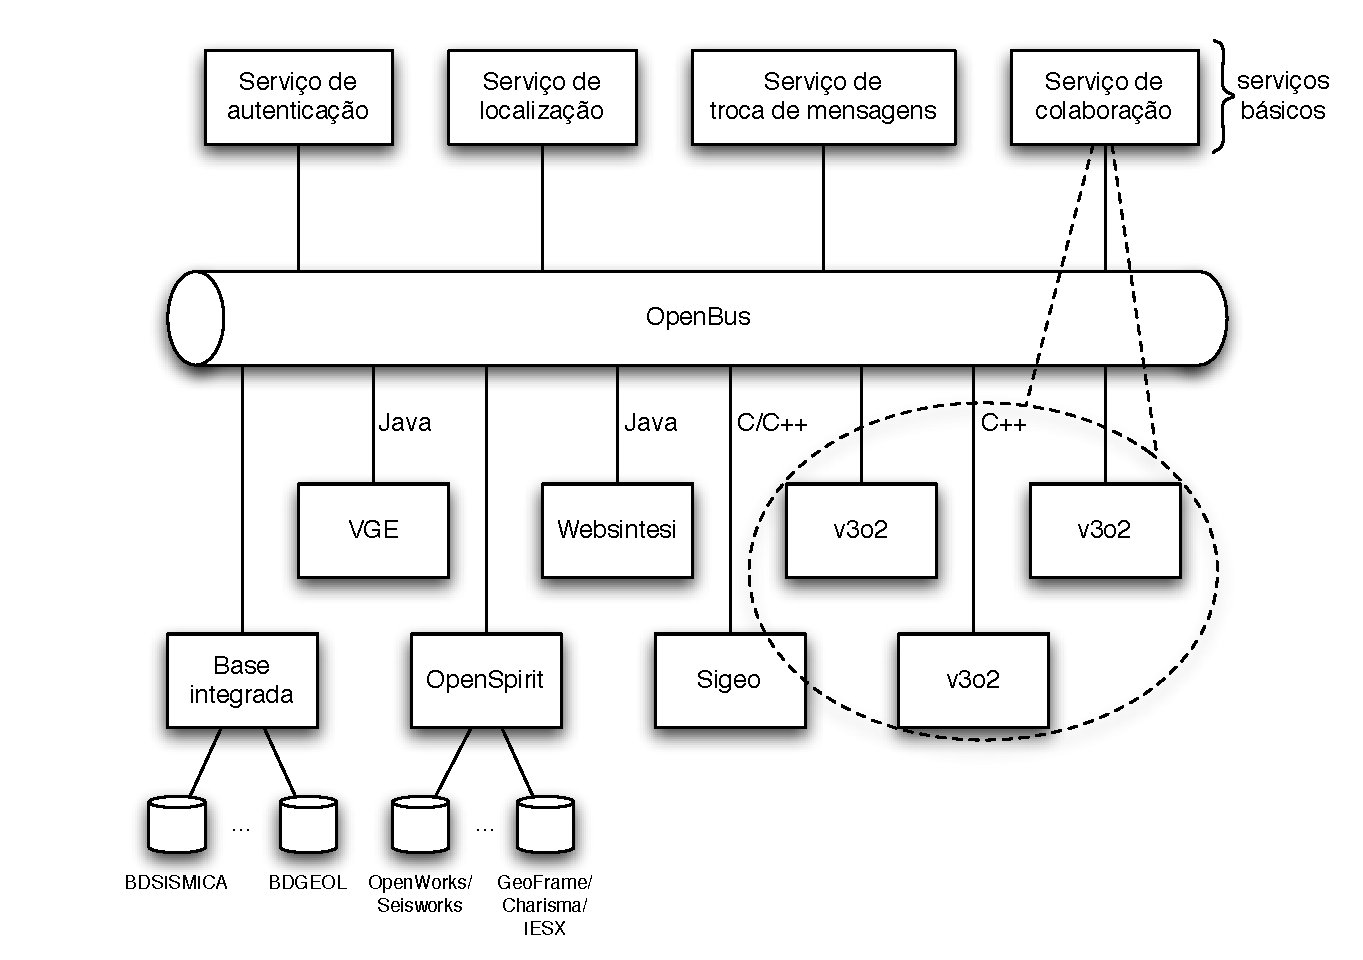
\includegraphics[width=14cm]{figs/arquitetura.pdf} %height=3in, 
\caption{Arquitetura do \openbus}
\label{fig:architecture}
\end{figure}

Qualquer aplica��o que queira fazer parte do barramento deve
implementar um componente para o \openbus. Atrav�s desse componente
� poss�vel acessar todos os servi�os existentes no barramento.
Para isso, o componente deve ser capaz de se conectar ao barramento e se
autenticar.
Atrav�s dos servi�os oferecidos pelo \openbus, o componente pode acessar
um servi�o previamente conhecido, ou pode consultar o servi�o de
localiza��o para descobrir qual componente oferece o servi�o que ele
deseja acessar.
Para oferecer um servi�o, uma aplica��o pode usar o mesmo componente ou
implementar outro. Tal componente deve ser capaz de publicar no
barramento a interface do servi�o que deseja oferecer.

%\subsection{Servi�os b�sicos}

Entre os servi�os b�sicos oferecidos pelo \openbus\/ podemos destacar os
servi�os de autentica��o, localiza��o, troca de mensagens e colabora��o.

\begin{itemize}
%%%%%%%%%%
\item Servi�o de autentica��o 
%%%%%%%%%%

Para fazer parte do barramento, um componente deve se autenticar a ele.
Existem tipicamente duas formas de autentica��o para um
componente. Uma onde o componente usa a credencial de um usu�rio e outra
onde o componente (ou aplica��o) possui uma credencial pr�pria.

Aplica��es como o VGE, onde o usu�rio fornece seu identificador e sua
senha, podem usar a pr�pria credencial do usu�rio para 
autenticar seus componentes no barramento.
J� as aplica��es que executam como um {\em daemon} podem utilizar uma
credencial pr�pria.

Como apenas um componente do barramento pode acessar servi�os de outro
componente e todos os componentes do barramento j� foram autenticados,
os componentes do barramento s�o considerados confi�veis.
Entretanto, cabe a cada servi�o verificar se um componente possui a
devida autoriza��o para acessar seus servi�os.

%%%%%%%%%%
\item Servi�o de localiza��o 
%%%%%%%%%%

O servi�o de localiza��o � baseado no servi�o de {\em trading} de 
CORBA. Este servi�o facilita a oferta e o descobrimento de inst�ncias de
servi�os de tipos espec�ficos.
Com este servi�o, componentes podem publicar suas caracter�sticas
e outros componentes podem encontrar os servi�os desejados
atrav�s das caracter�sticas publicadas.

Para publicar um servi�o, um componente prov� ao servi�o de localiza��o
uma descri��o de seu servi�o e a sua localiza��o.
Para encontrar um servi�o, um componente pergunta ao servi�o
de localiza��o se existe algum servi�o com determinadas caracter�sticas.
O servi�o de localiza��o procura entre as descri��es que possui e
responde com a localiza��o da interface do servi�o selecionado.
O componente que solicitou o servi�o pode ent�o acess�-lo.

%%%%%%%%%%
\item Servi�o de troca de mensagens
%%%%%%%%%%

O servi�o de troca de mensagens � baseado no servi�o de notifica��o de 
CORBA.
Atrav�s dele, as aplica��es podem comunicar-se livremente,
trocando mensagens diretas ou registrando interesse em receber 
mensagens quando algum even\-to ocorre na outra aplica��o.

Quando duas aplica��es est�o vendo o mesmo dado e uma delas o altera, 
atrav�s desse servi�o, ela pode enviar uma mensagem para a outra
aplica��o para que ela atualize a sua c�pia do dado.

%\begin{figure} [htb]
%\centering
%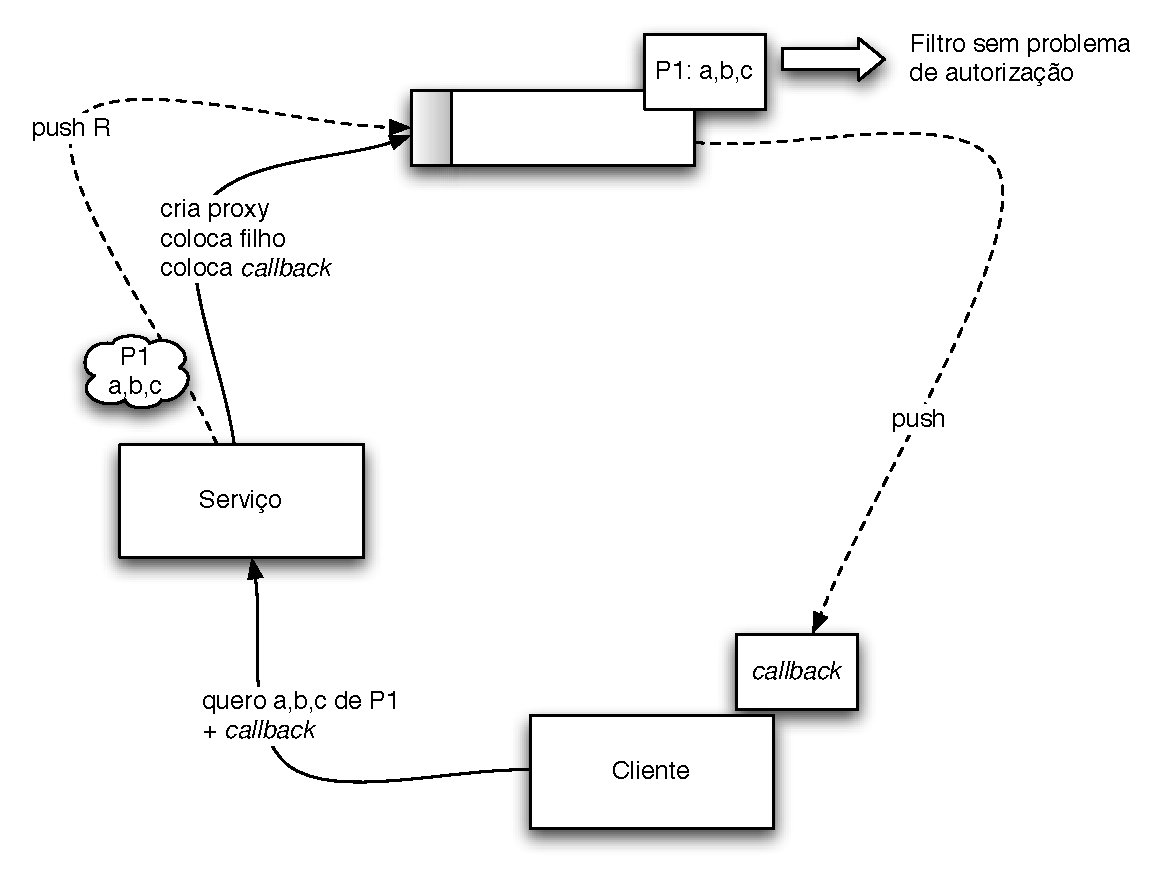
\includegraphics[width=8cm]{figs/eventos.pdf} %height=3in, 
%\caption{Troca de mensagens}
%\label{fig:datachange}
%\end{figure}

%%%%%%%%%%
\item Servi�o de colabora��o
%%%%%%%%%%

O servi�o de colabora��o usa o servi�o de troca de mensagens.
Atrav�s dele, um componente pode criar uma se��o de
colabora��o definir quem s�o os componentes participantes.
Inicialmente, cada componente � convidado pelo servi�o de colabora��o
a fazer parte desta se��o.

Cada se��o de colabora��o possui atributos espec�ficos e pode envolver
mais de um tipo de aplica��o de diferentes usu�rios.
Por exemplo, uma colabora��o entre diferentes inst�ncias 
do v3o2 pode ter atributos de c�mera, para que as diferentes inst�ncias
tenham a mesma vis�o do volume (Figura~\ref{fig:architecture}.)
Atrav�s de uma se��o, os componentes envolvidos podem compartilhar
diferentes tipos de eventos, como por exemplo, eventos de intera��o
de usu�rio (sele��o e altera��o de dados, movimenta��o de cursor). Cada
componente pode gerar e receber esses eventos.

\end{itemize}



\section{Conclus�es}
\label{conclusoes}

A integra��o entre as aplica��es da �rea de E\&P da Petrobras e, em especial,
 entre essas aplica��es e as bases de dados corporativas � uma necessidade
 clara para os fluxos de trabalho atuais.
Entre as diferentes formas de estabelecer esta integra��o, a mais adequada, em
 nossa opini�o, � atrav�s de um barramento comum de servi�os, o que ainda se
 mostra alinhado com as diretrizes corporativas da Companhia.
Atrav�s do barramento de servi�os, n�o apenas alcan�amos a integra��o b�sica,
 por c�pia de dados, mas tamb�m viabilizamos, na mesma infra-estrutura, formas
 mais ricas de integra��o, como a monitora��o de dados compartilhados e
 mecanismos de colabora��o.

As ferramentas dispon�veis no mercado, voltadas a este fim, n�o atendem aos
 r�gidos requisitos que a �rea de E\&P estabelece.
Em fun��o disso, propomos a constru��o de uma arquitetura de integra��o de
 aplica��es, baseada em um barramento de servi�os, que chamamos de \openbus.

Ap�s uma an�lise das tecnologias dispon�veis atualmente para a constru��o de
 uma arquitetura de servi�os, conclu�mos que a arquitetura \openbus\/ deve ser
 implementada sobre o {\em middleware} CORBA.
Essa escolha se justifica pelo fato de que CORBA oferece a forma mais adequada
 para implementar uma arquitetura de servi�os cujos componentes sejam
 heterog�neos e os requisitos de escalabilidade e desempenho sejam cr�ticos.
Em fun��o desses requisitos, e do contexto mais amplo da Petrobras, definimos
 que a arquitetura \openbus\/ dever�:

\begin{itemize}
\item Ser aberta e extens�vel a dom�nios fora do E\&P.
\item Permitir a troca de dados estruturados de forma adequada ao dom�nio.
\item Permitir a integra��o de aplica��es escritas em diferentes linguagens.
\item Facilitar a integra��o de provedores e consumidores de dados.
\item Permitir a troca de mensagens gen�ricas entre aplica��es.
\item Apresentar efici�ncia na troca de dados de grande volume.
\item Apresentar escalabilidade na troca de grandes volumes de mensagens.
\item Prover suporte a mecanismos de autentica��o e autoriza��o.
\item Prover suporte para a implementa��o de colabora��o.
\end{itemize}

A implementa��o da arquitetura dever� prover os servi�os b�sicos de
 autentica��o, localiza��o, mensageria e colabora��o de forma operacional, para
 que esta estrutura possa ser reutilizada em diferentes contextos da Companhia.
Dentro do foco no E\&P, esta estrutura ser� especializada para modelar os dados
 dos dom�nios de geologia e geof�sica.
Por fim, ser�o codificadas as pontes de liga��o da Base Integrada e das
 aplica��es WebSintesi, VGE, v3o2 e Sigeo que os conectar�o ao barramento,
 permitindo sua integra��o e servindo de prova de conceito para a arquitetura
 \openbus.


\end{document}
